% Five metal particles (FMP) in UO2: two-zone model. Model of V. Bellani (MSc thesis, 2026) and changes
% EC November 2026. Build: latexmk -pdf fmp_two_zones.tex (in this folder).
\documentclass[aspectratio=169,10pt]{beamer}

\usepackage[T1]{fontenc}
\usepackage{lmodern}
\usepackage{amsmath,amssymb}
\usepackage{booktabs,array}
\usepackage{graphicx}
\usepackage{tikz}
\usetikzlibrary{arrows.meta,calc,positioning,decorations.pathmorphing}

\graphicspath{{../figures/}{../calibration_two_zones/results/}}

% ---------------------------------------------------------------- colour code
\definecolor{vb}{RGB}{25,25,25}      % model of V. Bellani, unchanged
\definecolor{new}{RGB}{0,92,200}     % new or added, EC November 2026
\definecolor{mod}{RGB}{214,92,0}     % modified with respect to V. Bellani, EC November 2026
\definecolor{muted}{RGB}{110,110,110}
\definecolor{rule}{RGB}{200,200,200}

\newcommand{\NEW}[1]{\textcolor{new}{#1}}
\newcommand{\MOD}[1]{\textcolor{mod}{#1}}
\newcommand{\vbtag}[1]{\text{\scriptsize\textcolor{muted}{[VB #1]}}}
\newcommand{\newtag}{\text{\scriptsize\textcolor{new}{\textbf{new}}}}
\newcommand{\modtag}[1]{\text{\scriptsize\textcolor{mod}{\textbf{modified}, [VB #1]}}}
\newcommand{\was}[1]{{\scriptsize\textcolor{muted}{V.\,Bellani: #1}}}
\newcommand{\swatch}[1]{\tikz[baseline=-0.6ex]\fill[#1] (0,0) rectangle (0.22,0.22);}

% ---------------------------------------------------------------- minimal theme
\setbeamertemplate{navigation symbols}{}
\setbeamercolor{normal text}{fg=vb,bg=white}
\setbeamercolor{frametitle}{fg=vb}
\setbeamerfont{frametitle}{series=\bfseries,size=\large}
\setbeamercolor{title}{fg=vb}
\setbeamerfont{title}{series=\bfseries,size=\Large}
\setbeamercolor{structure}{fg=vb}
\setbeamertemplate{itemize items}{\textcolor{muted}{\raisebox{0.15ex}{\scriptsize$\bullet$}}}
\setbeamertemplate{frametitle}{\vspace{0.5em}\insertframetitle\par\vspace{-0.35em}{\color{rule}\rule{\textwidth}{0.4pt}}}
\setbeamertemplate{footline}{%
  \hbox to \paperwidth{\hspace{1.2em}\tiny\color{muted}%
    \swatch{vb} V.\,Bellani (thesis 2026), [VB x.y] = thesis eq.\quad
    \swatch{new} new, EC November 2026\quad
    \swatch{mod} modified, EC November 2026%
    \hfill FMP two-zone model\quad\insertframenumber/\inserttotalframenumber\hspace{1.2em}}\vspace{0.6em}}
\setlength{\abovedisplayskip}{4pt}
\setlength{\belowdisplayskip}{4pt}
\setlength{\abovedisplayshortskip}{2pt}
\setlength{\belowdisplayshortskip}{2pt}

\title{Five metal particles (FMP) in UO$_2$: two-zone model}
\subtitle{Model of V.\,Bellani (MSc thesis, Politecnico di Milano, 2026)\\and changes EC November 2026, SCIANTIX 2.5}
\author{Elisa Cappellari}
\date{4 November 2026}

\begin{document}

% =====================================================================================================
\begin{frame}[plain]
  \vspace{2.5em}
  {\usebeamerfont{title}\inserttitle\par}
  \vspace{0.6em}
  {\color{muted}\insertsubtitle\par}
  \vspace{1.5em}
  \insertauthor\par
  {\small\color{muted}\insertdate\par}
  \vspace{2.2em}
  {\small
  \swatch{vb}\; black: model of V.\,Bellani, unchanged, with the equation number of the thesis [VB x.y]\par\smallskip
  \swatch{new}\; \NEW{blue: new equation or assumption (EC November 2026)}\par\smallskip
  \swatch{mod}\; \MOD{orange: modified with respect to V.\,Bellani (EC November 2026)}, the original form in grey\par}
  \vspace{1.5em}
  {\scriptsize\color{muted}Code: \texttt{src/models/FiveMetalParticles.C}, \texttt{src/operations/SetPhaseDiagram.C};
  cases and scripts: \texttt{validation/metallicinclusions/}; local branch \texttt{development/metallicinclusionsv2.5}.}
\end{frame}

% =====================================================================================================
\begin{frame}{Changes with respect to the model of V.\,Bellani}
  \scriptsize
  \renewcommand{\arraystretch}{1.12}
  \begin{tabular}{@{}p{0.2\textwidth}p{0.33\textwidth}p{0.42\textwidth}@{}}
    \toprule
    Item & V.\,Bellani & EC November 2026 \\
    \midrule
    Production & lumped yield $y = 0.578$ at/fiss [VB 3.3] & \MOD{sum of the Mo, Tc, Ru, Rh, Pd systems, LWR yields, 0.5666 at/fiss} \\
    Matrix & one matrix, $C_m$ [VB 3.4] & \NEW{two zones: grain interior and grain-boundary zone ($\delta = 100$ nm), exchange $K_{\mathrm{ex}}$} \\
    Supersaturation & $S = C_m/C_{\mathrm{eq}}$ for both populations [VB 3.16] & \MOD{$S_k = c_k/C_{\mathrm{eq}}$ of the zone of each population} \\
    Intragranular sites & $f_d\rho_d/\lambda + f_b N_b$ [VB 3.29] & \MOD{same, times $\phi_1$} \\
    Nucleation mass limit & both requests reduced by $f_{\mathrm{mass}}$ [VB 4.10] & \MOD{each population limited by the metal of its zone} \\
    Implicit system & $3\times3$ [VB 4.17] & \MOD{$4\times4$ with the exchange} \\
    Parameters & common $k_0$, $B$ [VB 6.4, 6.5] & \MOD{free $k_{0}$ and $B$ for each population (new calibration)} \\
    Radius & from all the inventory [VB 3.49] & \MOD{from the metallic part, $\phi_{\mathrm{met}} = 1 - x_{\mathrm{Mo}} f_{\mathrm{ox}}$} \\
    OpenCalphad input & --- (all of ``X produced'' at the grain boundary) & \NEW{grain-boundary inventory $x_X C^{\mathrm{GB}}$, Mo oxide fraction $f_{\mathrm{ox}}$} \\
    Oxygen & not coupled & \NEW{balance fuel / Mo oxides (Mo/MoO$_2$ buffer)} \\
    $f_{A,\mathrm{GB}}$ & per fuel volume, not in the objective [VB 6.16, Sec.\,6.3] & \MOD{per volume of the grain-boundary zone, in the objective $J_4$} \\
    Calibration & 2 parameters, $E_{\mathrm{cal}} = 0.614$ [VB 7.3] & \MOD{4 parameters, $J_4 = 0.554$ ($J_3 = 0.598$)} \\
    Name, switch & 5MP / MFP, \texttt{iCm} & \MOD{FMP, \texttt{iFMP}} \\
    \bottomrule
  \end{tabular}
\end{frame}

% =====================================================================================================
\begin{frame}{Two particle populations, two zones}
  \begin{columns}[T]
    \begin{column}{0.47\textwidth}
      \centering
      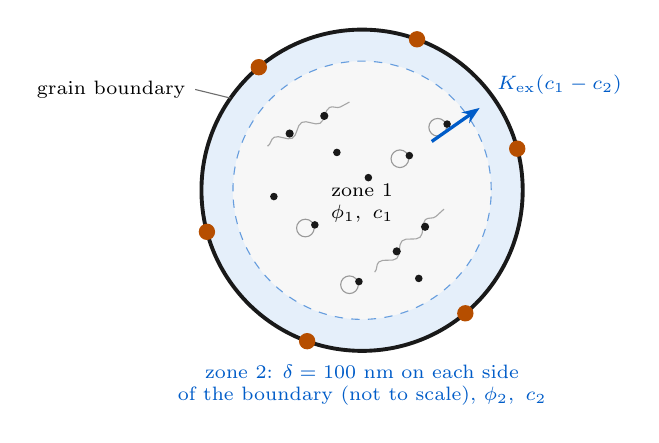
\begin{tikzpicture}[scale=0.8]
        % grain and grain-boundary zone (zone 2 not to scale)
        \fill[new!10] (0,0) circle (2.55);
        \fill[gray!6] (0,0) circle (2.05);
        \draw[new!60, dashed] (0,0) circle (2.05);
        \draw[line width=1.4pt, vb] (0,0) circle (2.55);
        % dislocation lines with particles
        \draw[gray!70, decorate, decoration={snake, amplitude=0.6mm, segment length=4mm}] (-1.5,0.7) -- (-0.2,1.4);
        \draw[gray!70, decorate, decoration={snake, amplitude=0.6mm, segment length=4mm}] (0.2,-1.3) -- (1.3,-0.3);
        \foreach \p in {(-1.15,0.9),(-0.6,1.18),(0.55,-0.97),(1.0,-0.58)} \fill[vb] \p circle (0.065);
        % intragranular bubbles with particles
        \foreach \bx/\by in {-0.9/-0.6, 0.6/0.5, -0.2/-1.5, 1.2/1.0} {\draw[gray!80] (\bx,\by) circle (0.14); \fill[vb] (\bx+0.15,\by+0.05) circle (0.06);}
        % isolated intragranular particles
        \foreach \p in {(0.1,0.2),(-1.4,-0.1),(0.9,-1.4),(-0.4,0.6)} \fill[vb] \p circle (0.06);
        % grain-boundary particles on the boundary
        \foreach \a in {15,70,130,195,250,310} \fill[mod!85!black] (\a:2.55) circle (0.13);
        % exchange arrow
        \draw[-{Stealth[length=2.2mm]}, line width=1.2pt, new] (35:1.35) -- (35:2.28);
        \node[new, font=\scriptsize, anchor=west, align=left] at (40:2.6) {$K_{\mathrm{ex}}(c_1-c_2)$};
        % labels
        \node[font=\scriptsize, align=center] at (0,-0.2) {zone 1\\$\phi_1,\ c_1$};
        \node[new, font=\scriptsize, align=center, anchor=north] at (0,-2.62) {zone 2: $\delta = 100$ nm on each side\\of the boundary (not to scale), $\phi_2,\ c_2$};
        \node[font=\scriptsize, anchor=east] at (-2.65,1.6) {grain boundary};
        \draw[muted] (-2.65,1.6) -- (145:2.55);
      \end{tikzpicture}
    \end{column}
    \begin{column}{0.5\textwidth}
      \footnotesize
      \textbf{Intragranular particles} $N_{\mathrm{intra}}, C^{\mathrm{intra}}, R_{\mathrm{intra}}$
      \begin{itemize}\footnotesize
        \item sites: dislocations ($f_d\rho_d/\lambda$) and intragranular bubbles ($f_b N_b$)
        \item fed by the metal dissolved in \NEW{zone 1, $c_1 = C_{m1}/\phi_1$}
      \end{itemize}
      \medskip
      \textbf{Grain-boundary particles} $N_{\mathrm{GB}}, C^{\mathrm{GB}}, R_{\mathrm{GB}}$
      \begin{itemize}\footnotesize
        \item sites: the boundary surface, $3/(2a\lambda^2)$
        \item fed by the metal dissolved in \NEW{zone 2, $c_2 = C_{m2}/\phi_2$}
      \end{itemize}
      \medskip
      \textbf{Processes}
      \begin{itemize}\footnotesize
        \item production \MOD{$\phi_k P$ in each zone}; nucleation (CNT); diffusion-limited growth
        \item re-solution, back \NEW{to the zone of the particles}
        \item \NEW{exchange between the zones, $K_{\mathrm{ex}}(c_1 - c_2)$}
      \end{itemize}
      \medskip
      {\footnotesize V.\,Bellani: one matrix $C_m$ feeds both populations with the same supersaturation
      (thesis Fig.\,3.1): with common parameters $R_{\mathrm{GB}} = R_{\mathrm{intra}}$ (thesis Tab.\,7.2).}
    \end{column}
  \end{columns}
\end{frame}

% =====================================================================================================
\begin{frame}{Metal balances: one matrix vs two zones}
  \begin{columns}[T]
    \begin{column}{0.44\textwidth}
      \centering
      {\small V.\,Bellani (thesis Fig.\,3.1, eqs.\,3.5--3.7)}\par\medskip
      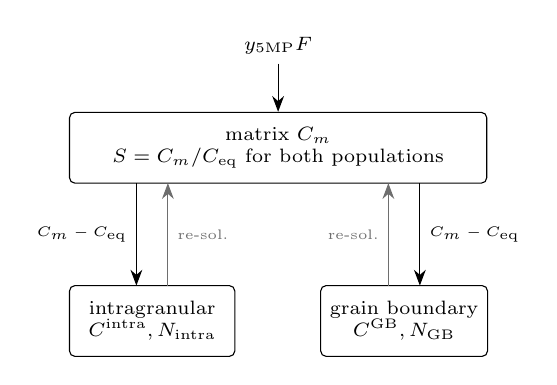
\begin{tikzpicture}[box/.style={draw, rounded corners=2pt, minimum width=2.1cm, minimum height=0.9cm, align=center, font=\scriptsize},
                          >={Stealth[length=2mm]}]
        \node[box, minimum width=5.3cm] (m) at (0,0) {matrix $C_m$\\$S = C_m/C_{\mathrm{eq}}$ for both populations};
        \node[box] (i) at (-1.6,-2.2) {intragranular\\$C^{\mathrm{intra}}, N_{\mathrm{intra}}$};
        \node[box] (g) at (1.6,-2.2) {grain boundary\\$C^{\mathrm{GB}}, N_{\mathrm{GB}}$};
        \node[font=\scriptsize] (p) at (0,1.3) {$y_{\mathrm{5MP}}F$};
        \draw[->] (p) -- (m);
        \draw[->] (-1.8,-0.45) -- node[left, font=\tiny] {$C_m - C_{\mathrm{eq}}$} (-1.8,-1.75);
        \draw[->, muted] (-1.4,-1.75) -- node[right, font=\tiny] {re-sol.} (-1.4,-0.45);
        \draw[->] (1.8,-0.45) -- node[right, font=\tiny] {$C_m - C_{\mathrm{eq}}$} (1.8,-1.75);
        \draw[->, muted] (1.4,-1.75) -- node[left, font=\tiny] {re-sol.} (1.4,-0.45);
      \end{tikzpicture}
    \end{column}
    \begin{column}{0.54\textwidth}
      \centering
      {\small \NEW{Two zones (EC November 2026)}}\par\medskip
      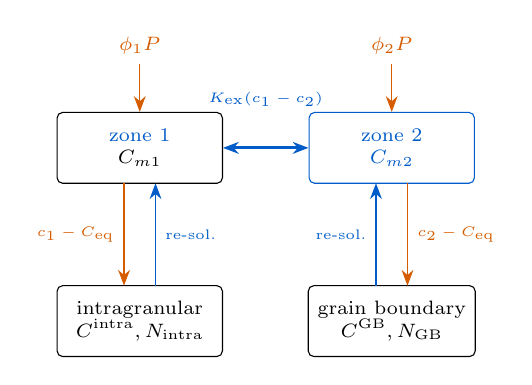
\begin{tikzpicture}[box/.style={draw, rounded corners=2pt, minimum width=2.1cm, minimum height=0.9cm, align=center, font=\scriptsize},
                          >={Stealth[length=2mm]}]
        \node[box] (m1) at (-1.6,0) {\NEW{zone 1}\\$C_{m1}$};
        \node[box, draw=new, text=new] (m2) at (1.6,0) {zone 2\\$C_{m2}$};
        \node[box] (i) at (-1.6,-2.2) {intragranular\\$C^{\mathrm{intra}}, N_{\mathrm{intra}}$};
        \node[box] (g) at (1.6,-2.2) {grain boundary\\$C^{\mathrm{GB}}, N_{\mathrm{GB}}$};
        \node[font=\scriptsize, mod] (p1) at (-1.6,1.3) {$\phi_1 P$};
        \node[font=\scriptsize, mod] (p2) at (1.6,1.3) {$\phi_2 P$};
        \draw[->, mod] (p1) -- (m1);
        \draw[->, mod] (p2) -- (m2);
        \draw[<->, new, line width=1pt] (m1) -- (m2);
        \node[new, font=\tiny] at (0,0.62) {$K_{\mathrm{ex}}(c_1 - c_2)$};
        \draw[->, mod] (-1.8,-0.45) -- node[left, font=\tiny] {$c_1 - C_{\mathrm{eq}}$} (-1.8,-1.75);
        \draw[->, new] (-1.4,-1.75) -- node[right, font=\tiny] {re-sol.} (-1.4,-0.45);
        \draw[->, mod] (1.8,-0.45) -- node[right, font=\tiny] {$c_2 - C_{\mathrm{eq}}$} (1.8,-1.75);
        \draw[->, new] (1.4,-1.75) -- node[left, font=\tiny] {re-sol.} (1.4,-0.45);
      \end{tikzpicture}
    \end{column}
  \end{columns}
  \vspace{0.8em}
  \small Total inventory conserved in both: production is the only net source [VB 3.8].
  \NEW{With the exchange the two populations see different concentrations, so the grain-boundary parameters can differ
  from the intragranular ones.}
\end{frame}

% =====================================================================================================
\begin{frame}{State variables}
  \scriptsize
  \renewcommand{\arraystretch}{1.15}
  \begin{tabular}{@{}l p{0.36\textwidth} l >{\ttfamily}p{0.33\textwidth}@{}}
    \toprule
    Symbol & Meaning & Unit & \normalfont SCIANTIX variable \\
    \midrule
    $C_{m1} + C_{m2}$ & metal dissolved in the UO$_2$ matrix [VB Tab.\,3.1, $C_m$] & at/m$^3$ & FMP in matrix \\
    \NEW{$C_{m2}$} & \NEW{metal dissolved in the grain-boundary zone} & at/m$^3$ & FMP in grain-boundary zone matrix \\
    $C^{\mathrm{intra}}$ & metal in intragranular particles & at/m$^3$ & FMP in intragranular particles \\
    $C^{\mathrm{GB}}$ & metal in grain-boundary particles & at/m$^3$ & FMP at grain boundary \\
    $N_{\mathrm{intra}}$, $N_{\mathrm{GB}}$ & particle number densities (per fuel volume) & FMP/m$^3$ & Intra-/Intergranular FMP concentration \\
    \MOD{$R_{\mathrm{intra}}$, $R_{\mathrm{GB}}$} & \MOD{mean radii, output} (VB: atoms per particle) & m & Intra-/Intergranular FMP radius \\
    \NEW{$\phi_2$} & \NEW{volume fraction of the grain-boundary zone} & -- & FMP grain-boundary zone volume fraction \\
    \NEW{$O_{\mathrm{ox}}$} & \NEW{oxygen in the Mo oxides of the particles} & at/m$^3$ & FMP oxygen in Mo oxides \\
    \NEW{$f_{\mathrm{ox}}$} & \NEW{fraction of the grain-boundary Mo in oxide phases (OpenCalphad)} & -- & Mo in oxide fraction \\
    \bottomrule
  \end{tabular}
  \vspace{0.8em}

  Inputs from SCIANTIX: temperature $T$, fission rate $F$, burnup $b$, grain radius $a$, intragranular bubble concentration
  $N_{b}$ (one-way coupling, [VB Sec.\,3.2]). The five metals are one lumped species [VB Sec.\,3.2].
\end{frame}

% =====================================================================================================
\begin{frame}{Production and inventory}
  \small
  V.\,Bellani: lumped yield from the PRODHEL composition (Angleraud), $x_{\mathrm{5MP}} = 0.289$ [VB 3.2]
  \begin{align*}
    \dot C_{\mathrm{5MP}} &= y_{\mathrm{5MP}} F, \qquad y_{\mathrm{5MP}} = 2 x_{\mathrm{5MP}} = 0.578\ \text{at/fiss} \tag*{\vbtag{3.1, 3.3}}
  \end{align*}
  \MOD{Now: sum of the five element systems ``X in UO$_2$'' (\texttt{SetSystem.C}), ENDF/B-VIII.0 yields with the fission
  fractions of an LWR cycle}
  \begin{align*}
    \MOD{\frac{dC_{\mathrm{FMP}}}{dt} = \sum_{X} y_X F,\quad X = \mathrm{Mo, Tc, Ru, Rh, Pd}} \tag*{\modtag{3.1}}
  \end{align*}
  \begin{center}\footnotesize
  \MOD{\begin{tabular}{cccccc}
    $y_{\mathrm{Mo}}$ & $y_{\mathrm{Tc}}$ & $y_{\mathrm{Ru}}$ & $y_{\mathrm{Rh}}$ & $y_{\mathrm{Pd}}$ & total \\
    0.2370 & 0.0614 & 0.1442 & 0.0469 & 0.0771 & 0.5666 at/fiss
  \end{tabular}}
  \end{center}
  \begin{align*}
    \NEW{x_X = \frac{C_X^{\mathrm{prod}}}{\sum_X C_X^{\mathrm{prod}}}}\quad \NEW{\text{(42Mo-11Tc-25Ru-8Rh-14Pd at.\%)}} \tag*{\newtag}\\
    \sum_X C_X^{\mathrm{prod}} = \MOD{C_{m1} + C_{m2}} + C^{\mathrm{intra}} + C^{\mathrm{GB}} \tag*{\modtag{3.4}}
  \end{align*}
  \was{$C_{\mathrm{5MP}} = C_m + C^{\mathrm{intra}} + C^{\mathrm{GB}}$.} The particle composition is the production
  composition $x_X$ (lumped species).
\end{frame}

% =====================================================================================================
\begin{frame}{Grain-boundary zone}
  \small
  \NEW{Zone 2 = shell of thickness $\delta$ inside each spherical grain of radius $a$, so that every boundary has a layer
  $\delta$ on both sides; zone 1 = grain interior.}
  \begin{align*}
    \NEW{\phi_2 = 1 - \left(1 - \frac{\delta}{a}\right)^3 \approx \frac{3\delta}{a}\ (\le 0.999),\qquad \phi_1 = 1 - \phi_2,
    \qquad \delta = 100\ \text{nm}} \tag*{\newtag}\\
    \NEW{P_k = \phi_k\,\Delta C_{\mathrm{prod}}\ \text{(uniform production)},\qquad c_k = \frac{C_{mk}}{\phi_k}\ \text{(local concentration)},\qquad k = 1, 2} \tag*{\newtag}
  \end{align*}
  \begin{itemize}
    \item \NEW{$\delta$ = half-width of the grain-boundary regions analysed by TEM in the calibration (strips of about
      200 nm across the boundary, thesis Figs.\,5.3--5.16)}
    \item calibration cases: $a = 12.3\ \mu$m $\Rightarrow \phi_2 = 0.024$; ATM-109: $a = 15\ \mu$m $\Rightarrow \phi_2 = 0.020$
    \item \NEW{no new fitted parameter}: $\delta$ comes from the TEM regions, the exchange from diffusion (below)
  \end{itemize}
\end{frame}

% =====================================================================================================
\begin{frame}{Equilibrium concentration and supersaturation}
  \small
  \begin{align*}
    C_{\mathrm{eq}}(T) &= C_{\mathrm{eq,ref}} \exp\left[-\frac{H_{\mathrm{sol}}^{\mathrm{eff}}}{k_B}\left(\frac{1}{T} - \frac{1}{T_{\mathrm{ref}}}\right)\right],
      \qquad T_{\mathrm{ref}} = 2173.15\ \text{K} \tag*{\vbtag{3.10, 3.11}}\\
    C_{\mathrm{eq,ref}} &= x_{\mathrm{eq,ref}} \frac{4}{a_{\mathrm{UO_2}}^3} = 6\times10^{-5} \cdot 2.437\times10^{28}
      = 1.462\times10^{24}\ \text{at/m}^3, \qquad H_{\mathrm{sol}}^{\mathrm{eff}} = 1.14\ \text{eV} \tag*{\vbtag{3.12--3.15}}
  \end{align*}
  Mo solubility in UO$_2$ at 1900\,$^\circ$C (Kleykamp), $a_{\mathrm{UO_2}} = 547.5$ pm, DFT solution energy of Mo (Brillant et al.).
  \medskip

  Supersaturation after the production of the time step:
  \begin{align*}
    S &= \frac{C_m^{n} + \Delta C_{\mathrm{prod}}}{C_{\mathrm{eq}}(T)} \tag*{\vbtag{4.2, 4.3}}\\
    \MOD{S_k} &\MOD{= \frac{C_{mk}^{n} + \phi_k \Delta C_{\mathrm{prod}}}{\phi_k\, C_{\mathrm{eq}}(T)} = \frac{c_k^{*}}{C_{\mathrm{eq}}},\qquad
      k = 1 \text{ for the intragranular}, \ k = 2 \text{ for the grain-boundary particles}} \tag*{\modtag{3.16, 4.3}}\\
    \Delta\mu_k &= k_B T \ln S_k \quad (S_k > 1;\ \text{no nucleation for } S_k \le 1) \tag*{\vbtag{3.17}}
  \end{align*}
\end{frame}

% =====================================================================================================
\begin{frame}{Nucleation: classical nucleation theory}
  \small
  Heterogeneous nucleation, capillarity approximation, $j = $ intra, GB with \MOD{$S$ of the zone of the population}:
  \begin{align*}
    \Delta G_j^{*} &= \frac{B_j}{T^2 (\ln \MOD{S_k})^2}, \qquad B_j = \frac{16\pi\gamma_j^3\Omega_{\mathrm{5MP}}^2\Phi_j}{3k_B^2}
      \ \text{(effective, calibrated)} \tag*{\vbtag{3.20, 3.21}}\\
    k_{\mathrm{nucl},j} &= k_{\mathrm{nucl},0,j} \exp\left(-\frac{\Delta G_j^{*}}{k_B T}\right), \qquad k_{\mathrm{nucl},0,j} = 1\ \text{s}^{-1} \tag*{\vbtag{3.22}}\\
    \frac{dN_j}{dt} &= k_{\mathrm{nucl},j} \max\left(N_{\mathrm{site},j} - N_j, 0\right) \tag*{\vbtag{3.9}}
  \end{align*}
  Backward Euler, $N_j$ never decreases:
  \begin{align*}
    N_j^{n+1,*} = \frac{N_j^n + k_{\mathrm{nucl},j} N_{\mathrm{site},j}\Delta t}{1 + k_{\mathrm{nucl},j}\Delta t},
      \qquad \Delta N_j = \max\left(N_j^{n+1,*} - N_j^n, 0\right) \tag*{\vbtag{4.5, 4.6}}
  \end{align*}
  \MOD{$B_{\mathrm{intra}} \ne B_{\mathrm{GB}}$, calibrated separately.} \was{$B_{\mathrm{intra}} = B_{\mathrm{GB}} = B_{\mathrm{ref}} s_B$,
  $s_{B,\mathrm{intra}} = s_{B,\mathrm{GB}}$ [VB 6.2, 6.4].}
\end{frame}

% =====================================================================================================
\begin{frame}{Nucleation sites}
  \small
  Intragranular: dislocations (Veshchunov and Shestak) and intragranular fission gas bubbles
  \begin{align*}
    \rho_d &= A\, b^{n} f_T, \qquad f_T = A_\infty + \frac{1 - A_\infty}{1 + \exp[(T - T_c)/\Delta T]} \tag*{\vbtag{3.23, 3.24}}\\
    &A = 6.545\times10^{12},\ n = 1.151,\ A_\infty = 0.608,\ T_c = 1109\ \text{K},\ \Delta T = 25.8\ \text{K},\ b\ \text{in MWd/kgUO}_2 \tag*{\vbtag{3.25}}\\
    N_{\mathrm{site,intra}} &= \MOD{\phi_1}\left(f_d\frac{\rho_d}{\lambda} + f_b N_{b,\mathrm{intra}}\right),
      \qquad f_d = 0.67,\ f_b = 0.33,\ \lambda = 15\ \text{nm} \tag*{\modtag{3.29}}
  \end{align*}
  \MOD{Factor $\phi_1$: the intragranular sites are in zone 1 only.} \was{no factor.}
  \medskip

  Grain boundary: the boundary surface, area per unit volume $3/(2a)$ (each boundary shared by two grains), one site every $\lambda^2$
  \begin{align*}
    N_{\mathrm{site,GB}} = \frac{A_{\mathrm{GB}}}{V}\frac{1}{\lambda^2} = \frac{3}{2a\lambda^2} \tag*{\vbtag{3.31--3.33}}
  \end{align*}
  {\footnotesize End of r000 (54.1 MWd/kgUO$_2$): dislocation sites $2.2\times10^{22}$, bubble sites $1.4\times10^{23}$,
  $N_{\mathrm{intra}} = 5.8\times10^{21}$; GB sites $5.4\times10^{20}$, $N_{\mathrm{GB}} = 3.2\times10^{19}$ m$^{-3}$
  (4--6\% of the sites occupied).}
\end{frame}

% =====================================================================================================
\begin{frame}{Metal taken by nucleation}
  \small
  Atoms per nucleus: critical size of CNT, at least a dimer (Ru clusters in UO$_2$)
  \begin{align*}
    n_{\mathrm{nucl},j} = \max\left(2, \frac{2\Delta G_j^{*}}{\Delta\mu}\right), \qquad \Delta C_{\mathrm{nucl},j} = n_{\mathrm{nucl},j}\,\Delta N_j \tag*{\vbtag{3.34--3.36, 4.7, 4.8}}
  \end{align*}
  V.\,Bellani: the two requests are limited together by the dissolved metal, in proportion
  \begin{align*}
    \text{if } \Delta C_{\mathrm{nucl,intra}} + \Delta C_{\mathrm{nucl,GB}} > C_m^{\mathrm{avail}}:\quad
    f_{\mathrm{mass}} = \frac{C_m^{\mathrm{avail}}}{\Delta C_{\mathrm{nucl,intra}} + \Delta C_{\mathrm{nucl,GB}}},\quad
    \Delta C^{\mathrm{act}}_{\mathrm{nucl},j} = f_{\mathrm{mass}}\Delta C_{\mathrm{nucl},j} \tag*{\vbtag{4.9--4.11}}
  \end{align*}
  \MOD{Now: each population takes the atoms of its own zone ($k = 1$ for intra, $k = 2$ for GB)}
  \begin{align*}
    \MOD{\Delta C^{\mathrm{act}}_{\mathrm{nucl},j} = \min\left(n_{\mathrm{nucl},j}\Delta N_j,\ C_{mk}^{n} + \phi_k\Delta C_{\mathrm{prod}}\right)} \tag*{\modtag{4.9--4.11}}\\
    \Delta N_j^{\mathrm{act}} = \frac{\Delta C^{\mathrm{act}}_{\mathrm{nucl},j}}{n_{\mathrm{nucl},j}}, \qquad
    N_j^{n+1} = N_j^n + \Delta N_j^{\mathrm{act}} \tag*{\vbtag{4.12}}
  \end{align*}
\end{frame}

% =====================================================================================================
\begin{frame}{Growth (precipitation)}
  \small
  Diffusion-limited capture by spherical particles, $4\pi D R$ per particle (Ham; Brailsford et al.)
  \begin{align*}
    k_j &= D_j\, 4\pi N_j R_j, \qquad D_j = k_{0,j} \exp\left(-\frac{\Delta G_j}{k_B T}\right),
      \qquad \Delta G_{\mathrm{intra}} = \Delta G_{\mathrm{GB}} = 1\ \text{eV} \tag*{\vbtag{3.38, 3.39}}
  \end{align*}
  evaluated with the state at the beginning of the time step (no iteration on $R \to k \to C$) [VB 4.13].
  \begin{align*}
    J_{\mathrm{prec},j} &= k_j \max\left(C_m - C_{\mathrm{eq}}, 0\right) \tag*{\vbtag{3.37}}\\
    \MOD{J_{\mathrm{prec,intra}}} &\MOD{= k_{\mathrm{intra}}\,(c_1 - C_{\mathrm{eq}}),\qquad J_{\mathrm{prec,GB}} = k_{\mathrm{GB}}\,(c_2 - C_{\mathrm{eq}})} \tag*{\modtag{3.37}}
  \end{align*}
  \MOD{each active only if its zone is supersaturated after production and nucleation, $c_k^{*} > C_{\mathrm{eq}}$}
  (V.\,Bellani: both active if $C_m^{*} > C_{\mathrm{eq}}$ [VB 4.19]). No thermal dissolution [VB Sec.\,3.5].
  \medskip

  \MOD{$k_{0,\mathrm{intra}} \ne k_{0,\mathrm{GB}}$, calibrated separately: $D_{\mathrm{GB}}/D_{\mathrm{intra}} = 3.06$.}
  \was{common $k_0$, $s_{k0,\mathrm{intra}} = s_{k0,\mathrm{GB}}$ [VB 6.5].}
\end{frame}

% =====================================================================================================
\begin{frame}{Exchange between the zones}
  \small
  \NEW{Flux from zone 1 to zone 2 per unit fuel volume: $J_{\mathrm{ex}} = K_{\mathrm{ex}}(c_1 - c_2)$, two resistances in series:
  grain interior $\to$ interface (grain-boundary sink strength with the intragranular particles as internal sinks),
  interface $\to$ middle of zone 2 (distance $\delta/2$, area $3/a$ per unit volume).}
  \begin{align*}
    \NEW{K_{\mathrm{ex}} = \frac{D_{\mathrm{intra}}}{1/k_{\mathrm{GB}}^2 + a\delta/6},\qquad
    k_{\mathrm{GB}}^2 = \max\left(k_1^2\frac{F}{1-F}, \frac{15}{a^2}\right),\qquad
    F = \frac{3}{z}\left(\coth z - \frac{1}{z}\right),\quad z = k_1 a} \tag*{\newtag}\\
    \NEW{k_1^2 = 4\pi\frac{N_{\mathrm{intra}}}{\phi_1}R_{\mathrm{intra}}\quad\text{(sink strength of the intragranular particles in zone 1)}} \tag*{\newtag}
  \end{align*}
  \NEW{Equivalent Fick form: area $\times$ $D$ $/$ distance}
  \begin{align*}
    \NEW{K_{\mathrm{ex}} = \frac{3}{a}\,\frac{D_{\mathrm{intra}}}{L_1 + \delta/2},\qquad L_1 = \frac{3}{a k_{\mathrm{GB}}^2} =
    \begin{cases} a/5 = 2.5\ \mu\text{m} & \text{no particles (Booth sphere)}\\ \approx 1/k_1 & \text{particles dominate, } z \gg 1\end{cases}} \tag*{\newtag}
  \end{align*}
  \NEW{$1/k_1$ = distance travelled by a dissolved atom before the capture by a particle.} r000: $L_1$ = 107 nm at 14 and
  42 nm at 54.1 MWd/kgUO$_2$, against $\delta/2 = 50$ nm. \NEW{No new parameter.}
\end{frame}

% =====================================================================================================
\begin{frame}{Exchange: derivation}
  \begin{columns}[T]
    \begin{column}{0.5\textwidth}
      \footnotesize
      \NEW{\textbf{1.} Sphere of radius $a$, uniform source $S$, particles as uniform sinks $k_1^2$, interface concentration $c_i$,
      $u = c - c_i$, quasi-steady state:}
      \[\NEW{D\,\frac{1}{r^2}\frac{d}{dr}\!\left(r^2\frac{du}{dr}\right) - Dk_1^2u + S = 0,\quad u'(0) = 0,\ u(a) = 0}\]
      \[\NEW{u(r) = \frac{S}{Dk_1^2}\left[1 - \frac{a\sinh(k_1r)}{r\sinh(k_1a)}\right]}\]
      \NEW{\textbf{2.} Mean, with $\int_0^a r\sinh(k_1r)\,dr = \frac{a\cosh z}{k_1} - \frac{\sinh z}{k_1^2}$, $z = k_1a$:}
      \[\NEW{\bar u = \frac{3}{a^3}\int_0^a u\,r^2dr = \frac{S}{Dk_1^2}(1 - F),\quad F = \frac{3}{z}\left(\coth z - \frac{1}{z}\right)}\]
      \NEW{\textbf{3.} The source goes to the particles or across $r = a$: $S = Dk_1^2\bar u + Dk_{\mathrm{GB}}^2\bar u$}
      \[\NEW{k_{\mathrm{GB}}^2 = \frac{k_1^2}{1-F} - k_1^2 = k_1^2\frac{F}{1-F}}\]
    \end{column}
    \begin{column}{0.48\textwidth}
      \footnotesize
      \NEW{\textbf{4.} Limits: $z\to0$: $\coth z = 1/z + z/3 - z^3/45$, $F = 1 - z^2/15$, $k_{\mathrm{GB}}^2 \to 15/a^2$ (Booth sphere,
      $\bar u = Sa^2/15D$); $z\gg1$: $F\approx3/z$, $k_{\mathrm{GB}}^2\to3k_1/a$.}\par\smallskip
      \NEW{\textbf{5.} Interface $\to$ middle of zone 2, area $4\pi a^2/(\frac{4}{3}\pi a^3) = 3/a$:}
      \[\NEW{J = \frac{3}{a}\,\frac{D(c_i - c_2)}{\delta/2} = \frac{6D}{a\delta}(c_i - c_2)}\]
      \NEW{\textbf{6.} Series: $c_1 - c_i = J/(Dk_{\mathrm{GB}}^2)$, $c_i - c_2 = Ja\delta/(6D)$, summing:}
      \[\NEW{J = \frac{D(c_1 - c_2)}{1/k_{\mathrm{GB}}^2 + a\delta/6} = K_{\mathrm{ex}}(c_1 - c_2)}\]
      \textbf{Exact}: steps 1--4, for any $c_i$ and with the $C_{\mathrm{eq}}$ term (only $S$ changes).\par
      \textbf{Approximate}: zone 2 well mixed with its mean at $\delta/2$; radius $a$ instead of $a - \delta$ (0.8\%);
      $D_{\mathrm{intra}}$ also in zone 2; quasi-steady state at each step. Code block marked [TBC].
      {\scriptsize Brailsford and Bullough (1981); Booth (1957).}
    \end{column}
  \end{columns}
\end{frame}

% =====================================================================================================
\begin{frame}{Exchange: numerical check}
  \centering
  \includegraphics[width=0.9\textwidth]{exchange_check.png}\par\medskip
  \small
  \begin{itemize}
    \item left: profile in the grain, without particles and with the particles of r000 at 54.1 MWd/kgUO$_2$ ($z = 293$):
      only the metal produced in the last $\sim$40 nm reaches the boundary
    \item right: $k_{\mathrm{GB}}^2a^2$ from a finite-volume solution of step 1 vs the expression of step 3, agreement within
      $6\times10^{-8}$ for $z = 0.1$--293, and the two limits of step 4 (\texttt{check\_exchange.py})
  \end{itemize}
\end{frame}

% =====================================================================================================
\begin{frame}{Irradiation-induced re-solution}
  \small
  First order in the precipitated inventory, same coefficient for the two populations
  \begin{align*}
    J_{\mathrm{res},j} = k_{\mathrm{res}}\,C^{j} \tag*{\vbtag{3.40}}
  \end{align*}
  From the shrinkage of the FMP under ion irradiation (Sakib et al. 2025): $R_1/R_0 = 0.80/0.91$ between 0.30 and 1.75 dpa,
  $n\propto R^3$, $\dot D_{\mathrm{ref}} = 1$ dpa/day
  \begin{align*}
    k_{\mathrm{res}} = -\frac{3}{\Delta t}\ln\frac{R_1}{R_0},\quad \Delta t = \frac{\Delta D}{\dot D_{\mathrm{ref}}} \;\Rightarrow\;
    k_{\mathrm{res,ref}} = 3.085\times10^{-6}\ \text{s}^{-1} \tag*{\vbtag{3.41--3.45}}\\
    k_{\mathrm{res}}(F) = k_{\mathrm{res,ref}}\frac{F}{F_{\mathrm{ref}}},\qquad F_{\mathrm{ref}} = 1.48\times10^{19}\ \text{fiss/(m}^3\,\text{s)} \tag*{\vbtag{3.46, 3.47}}
  \end{align*}
  \NEW{The re-solved metal returns to the zone of the particles: intragranular $\to$ zone 1, grain boundary $\to$ zone 2.}
  \was{to the single matrix.}
\end{frame}

% =====================================================================================================
\begin{frame}{Metal balance: one matrix $\to$ two zones}
  \small
  V.\,Bellani, continuous form [VB 3.5--3.7] and backward-Euler $3\times3$ system, $\mathbf{C} = (C_m, C^{\mathrm{intra}}, C^{\mathrm{GB}})$ [VB 4.15--4.18]:
  \begin{align*}
    \frac{dC_m}{dt} &= y_{\mathrm{5MP}}F - J_{\mathrm{nucl,intra}} - J_{\mathrm{nucl,GB}} - (k_{\mathrm{intra}} + k_{\mathrm{GB}})(C_m - C_{\mathrm{eq}}) + k_{\mathrm{res}}(C^{\mathrm{intra}} + C^{\mathrm{GB}}) \tag*{\vbtag{3.5}}
  \end{align*}
  \[\footnotesize \begin{pmatrix} 1 + (k_{\mathrm{intra}} + k_{\mathrm{GB}})\Delta t & -k_{\mathrm{res}}\Delta t & -k_{\mathrm{res}}\Delta t\\
     -k_{\mathrm{intra}}\Delta t & 1 + k_{\mathrm{res}}\Delta t & 0\\ -k_{\mathrm{GB}}\Delta t & 0 & 1 + k_{\mathrm{res}}\Delta t\end{pmatrix}
     \mathbf{C}^{n+1} = \begin{pmatrix} C_m^{*} + (k_{\mathrm{intra}} + k_{\mathrm{GB}})C_{\mathrm{eq}}\Delta t\\ C^{\mathrm{intra},*} - k_{\mathrm{intra}}C_{\mathrm{eq}}\Delta t\\ C^{\mathrm{GB},*} - k_{\mathrm{GB}}C_{\mathrm{eq}}\Delta t\end{pmatrix}
     \tag*{\vbtag{4.17, 4.18}}\]
  \MOD{Now, after production and nucleation, $\mathbf{C} = (C_{m1}, C_{m2}, C^{\mathrm{intra}}, C^{\mathrm{GB}})$:}
  \begin{align*}
    \MOD{\frac{dC_{m1}}{dt}} &\MOD{= - k_{\mathrm{intra}}(c_1 - C_{\mathrm{eq}}) - K_{\mathrm{ex}}(c_1 - c_2) + k_{\mathrm{res}}C^{\mathrm{intra}}} \tag*{\modtag{3.5}}\\
    \MOD{\frac{dC_{m2}}{dt}} &\MOD{= - k_{\mathrm{GB}}(c_2 - C_{\mathrm{eq}}) + K_{\mathrm{ex}}(c_1 - c_2) + k_{\mathrm{res}}C^{\mathrm{GB}}} \tag*{\newtag}\\
    \frac{dC^{\mathrm{intra}}}{dt} &= k_{\mathrm{intra}}(\MOD{c_1} - C_{\mathrm{eq}}) - k_{\mathrm{res}}C^{\mathrm{intra}},\qquad
    \frac{dC^{\mathrm{GB}}}{dt} = k_{\mathrm{GB}}(\MOD{c_2} - C_{\mathrm{eq}}) - k_{\mathrm{res}}C^{\mathrm{GB}} \tag*{\modtag{3.6, 3.7}}
  \end{align*}
  production ($P_k$) and nucleation are applied before, as in [VB 4.2, 4.14].
\end{frame}

% =====================================================================================================
\begin{frame}{Implicit $4\times4$ system}
  \small
  \MOD{Backward Euler (\texttt{Solver::Laplace}), $\kappa_1 = k_{\mathrm{intra}}$ if $c_1^{*} > C_{\mathrm{eq}}$ else 0,
  $\kappa_2 = k_{\mathrm{GB}}$ if $c_2^{*} > C_{\mathrm{eq}}$ else 0 ($^*$ = after production and nucleation):}
  \[\MOD{\begin{pmatrix}
    1 + \frac{(\kappa_1 + K_{\mathrm{ex}})\Delta t}{\phi_1} & -\frac{K_{\mathrm{ex}}\Delta t}{\phi_2} & -k_{\mathrm{res}}\Delta t & 0\\[4pt]
    -\frac{K_{\mathrm{ex}}\Delta t}{\phi_1} & 1 + \frac{(\kappa_2 + K_{\mathrm{ex}})\Delta t}{\phi_2} & 0 & -k_{\mathrm{res}}\Delta t\\[4pt]
    -\frac{\kappa_1\Delta t}{\phi_1} & 0 & 1 + k_{\mathrm{res}}\Delta t & 0\\[4pt]
    0 & -\frac{\kappa_2\Delta t}{\phi_2} & 0 & 1 + k_{\mathrm{res}}\Delta t
  \end{pmatrix}
  \begin{pmatrix} C_{m1}\\ C_{m2}\\ C^{\mathrm{intra}}\\ C^{\mathrm{GB}}\end{pmatrix}^{n+1}
  = \begin{pmatrix} C_{m1}^{*} + \kappa_1C_{\mathrm{eq}}\Delta t\\ C_{m2}^{*} + \kappa_2C_{\mathrm{eq}}\Delta t\\
    C^{\mathrm{intra},*} - \kappa_1C_{\mathrm{eq}}\Delta t\\ C^{\mathrm{GB},*} - \kappa_2C_{\mathrm{eq}}\Delta t\end{pmatrix}}
  \tag*{\modtag{4.17, 4.18}}\]
  \begin{itemize}
    \item $1/\phi_k$: the fluxes depend on the local concentrations $c_k = C_{mk}/\phi_k$
    \item every column sums to 1: the total metal is conserved [VB 4.20]; checked on the outputs, inventory $= \sum_X C_X^{\mathrm{prod}}$
      within $4\times10^{-7}$ (the output precision)
    \item \MOD{growth switched on per zone} (V.\,Bellani: both on if $C_m^{*} > C_{\mathrm{eq}}$ [VB 4.19]); re-solution always active
  \end{itemize}
\end{frame}

% =====================================================================================================
\begin{frame}{Particle radius}
  \small
  Mean spherical-equivalent radius from the precipitated inventory and the number density
  \begin{align*}
    n_j = \frac{C^{j}}{N_j},\qquad R_j = \left(\frac{3 n_j\Omega_{\mathrm{5MP}}}{4\pi}\right)^{1/3} \tag*{\vbtag{3.48, 3.49}}\\
    \Omega_{\mathrm{5MP}} = \frac{V_w}{\eta_{\mathrm{hcp}}} = \frac{1.06651\times10^{-29}}{0.74} = 1.44123\times10^{-29}\ \text{m}^3/\text{at} \tag*{\vbtag{3.50--3.52}}
  \end{align*}
  ($V_w$: volumes of the atomic spheres, weights 40Mo:30Ru:10Tc:15Pd:5Rh, [VB Tab.\,3.2]).
  \medskip

  \MOD{Now, only the metallic part of the inventory (with OpenCalphad), $R_j = 0$ while $N_j < 1$ m$^{-3}$:}
  \begin{align*}
    \MOD{R_j = \left(\frac{3\,\phi_{\mathrm{met}}\,C^{j}\,\Omega_{\mathrm{5MP}}}{4\pi N_j}\right)^{1/3},\qquad
    \phi_{\mathrm{met}} = 1 - x_{\mathrm{Mo}}\,f_{\mathrm{ox}}} \tag*{\modtag{3.49}}
  \end{align*}
  \NEW{$\phi_{\mathrm{met}} = 1$ without thermochemistry; $f_{\mathrm{ox}}$ of the previous time step (next slide).}
  The radius is used in $k_j$ at the next step: $N_j, C^j \to R_j \to k_j \to C^j$ [VB Sec.\,3.6].
\end{frame}

% =====================================================================================================
\begin{frame}{Coupling with OpenCalphad at the grain boundary}
  \small
  \NEW{With \texttt{iThermochimica}, OpenCalphad at the grain boundary receives the grain-boundary inventory of the model:}
  \begin{align*}
    \NEW{n_X^{\mathrm{OC}} = x_X\,C^{\mathrm{GB}},\qquad X = \mathrm{Mo, Tc, Ru, Rh, Pd}} \tag*{\newtag}
  \end{align*}
  \MOD{instead of the whole production ``X produced'', which was also counted in the FMP reservoirs (double inventory).}
  \medskip

  \NEW{\texttt{JOGFormation} stores the fraction of this Mo in oxide phases (MoO$_2$, Mo$_4$O$_{11}$, \ldots):}
  \begin{align*}
    \NEW{f_{\mathrm{ox}} = \frac{\mathrm{Mo\ in\ oxide\ phases}}{n_{\mathrm{Mo}}^{\mathrm{OC}}},\qquad
    \phi_{\mathrm{met}} = 1 - x_{\mathrm{Mo}}\,f_{\mathrm{ox}}\ \text{(all the particles)}} \tag*{\newtag}
  \end{align*}
  \begin{itemize}
    \item \NEW{the oxygen potential is uniform in the grain: $f_{\mathrm{ox}}$ of the grain boundary holds for all the particles}
    \item \NEW{the oxidised Mo stays in the particle inventory (re-solved with it); one time step of lag}
    \item \NEW{a step where OpenCalphad gives no result keeps the previous $f_{\mathrm{ox}}$}
    \item database \texttt{BaMoO\_CsMoO\_MoPdRhRuTc\_merged.TDB} (Mo, O, Pd, Rh, Ru, Tc)
  \end{itemize}
\end{frame}

% =====================================================================================================
\begin{frame}{Oxygen balance between the fuel and the Mo oxides}
  \small
  \NEW{UO$_{2+x}$ with Kleykamp (1979) (\texttt{iStoichiometryDeviation = 7}, $\Delta x = 0.0013$ per \% FIMA). The excess oxygen $E$
  is shared between the fuel and the Mo oxides of the particles ($M$ = heavy-metal atoms per unit volume):}
  \begin{align*}
    \NEW{E = xM + O_{\mathrm{ox}},\qquad \mathrm{Mo}_p = x_{\mathrm{Mo}}(C^{\mathrm{intra}} + C^{\mathrm{GB}}),\qquad
    \mathrm{Mo}_{\mathrm{GB}} = x_{\mathrm{Mo}}C^{\mathrm{GB}}} \tag*{\newtag}
  \end{align*}
  \NEW{$E < 2\,\mathrm{Mo}_p$ --- Mo/MoO$_2$ buffer: OpenCalphad with the fixed oxygen $E\,\mathrm{Mo}_{\mathrm{GB}}/\mathrm{Mo}_p$ gives $\mu_{\mathrm{O}}$,
  then $x$ from Blackburn (Newton):}
  \begin{align*}
    \NEW{\ln\frac{p_{\mathrm{O_2}}}{1\ \text{atm}} = 2\ln\frac{x(2+x)}{1-x} + 108x^2 - \frac{32700}{T} + 9.92
    = \frac{2\mu_{\mathrm{O}}}{RT} + \ln\frac{1\ \text{bar}}{1\ \text{atm}},\quad x \le \frac{E}{M},\quad O_{\mathrm{ox}} = E - xM} \tag*{\newtag}
  \end{align*}
  \NEW{$E \ge 2\,\mathrm{Mo}_p$ --- all the Mo of the particles is MoO$_2$: $O_{\mathrm{ox}} = 2\,\mathrm{Mo}_p$,
  $x = (E - 2\,\mathrm{Mo}_p)/M$; OpenCalphad at the oxygen potential of the fuel.}
  \medskip

  \NEW{Then $x$, $p_{\mathrm{O_2}}$, $\mu_{\mathrm{O_2}}$ of the fuel are updated (Blackburn) and $\Delta O_{\mathrm{ox}}$ is removed from
  \texttt{O content}.} Without the balance: $x$ from Kleykamp and Mo oxidised without taking oxygen from the fuel.
  Only the Mo of the particles is an oxygen getter.
\end{frame}

% =====================================================================================================
\begin{frame}{Sequence in a time step}
  \small
  \begin{enumerate}
    \item production of the five systems (\texttt{FissionProductProduction}, \texttt{FissionProductDecay}) \MOD{[per element]}
    \item \NEW{$\phi_1$, $\phi_2$ from the grain radius; $P_k = \phi_k\Delta C_{\mathrm{prod}}$}
    \item $C_{\mathrm{eq}}(T)$; \MOD{$S_k$, $\Delta\mu_k$ per zone}
    \item nucleation sites ($\MOD{\phi_1}$ for the intragranular ones); $\Delta G^*_j$, $k_{\mathrm{nucl},j}$ with \MOD{$B_j$ per population}
    \item $\Delta N_j$ (backward Euler), $n_{\mathrm{nucl},j}$, metal of nucleation \MOD{limited by the zone}
    \item $R_j$, $k_j$ from the state at the beginning of the step (\MOD{$k_{0,j}$ per population}); \NEW{$K_{\mathrm{ex}}$}
    \item \MOD{$4\times4$ backward-Euler system}: growth, \NEW{exchange}, re-solution
    \item outputs: $C$'s, $N_j$, \MOD{$R_j$ with $\phi_{\mathrm{met}}$}, \NEW{$\phi_2$}
    \item \NEW{with thermochemistry: \texttt{SetPhaseDiagram} (OpenCalphad at the grain boundary with $x_X C^{\mathrm{GB}}$ and the
      oxygen balance), \texttt{JOGFormation} $\to f_{\mathrm{ox}}$ for the next step}
  \end{enumerate}
  \medskip
  {\footnotesize V.\,Bellani: steps 1--10 of thesis Sec.\,4.3 and Fig.\,4.1, routine \texttt{Simulation::MetallicFissionProducts()},
  switch \texttt{iCm}. \MOD{Now \texttt{FiveMetalParticles()}, switch \texttt{iFMP}.}}
\end{frame}

% =====================================================================================================
\begin{frame}{Parameters}
  \footnotesize
  \renewcommand{\arraystretch}{1.12}
  \begin{tabular}{@{}lll@{}}
    \toprule
    Parameter & Value & Origin \\
    \midrule
    \MOD{$k_{0,\mathrm{intra}}$} & \MOD{$9.834342\times10^{-16}$ m$^2$/s} & \MOD{calibrated} (VB: $4.980\times10^{-15}$, common [VB 7.2]) \\
    \MOD{$k_{0,\mathrm{GB}}$} & \MOD{$3.009503\times10^{-15}$ m$^2$/s} & \MOD{calibrated} (VB: $4.980\times10^{-15}$, common) \\
    \MOD{$B_{\mathrm{intra}}$} & \MOD{$2.711740\times10^{8}$ eV K$^2$} & \MOD{calibrated} (VB: $2.666\times10^{8}$, common [VB 7.2]) \\
    \MOD{$B_{\mathrm{GB}}$} & \MOD{$2.641409\times10^{8}$ eV K$^2$} & \MOD{calibrated} (VB: $2.666\times10^{8}$, common) \\
    $\Delta G_{\mathrm{intra}} = \Delta G_{\mathrm{GB}}$ & 1.0 eV & V.\,Bellani [VB 6.9] \\
    $k_{\mathrm{nucl},0,j}$ & 1.0 s$^{-1}$ & V.\,Bellani [VB 6.9] \\
    \NEW{$\delta$} & \NEW{100 nm} & \NEW{TEM grain-boundary regions (thesis Figs.\,5.3--5.16)} \\
    $\Omega_{\mathrm{5MP}}$ & $1.44123\times10^{-29}$ m$^3$/at & [VB 3.52] \\
    $n_{\min}$, $\lambda$ & 2 at, 15 nm & [VB 3.36, 3.27] \\
    $f_d$, $f_b$ & 0.67, 0.33 & image analysis [VB 3.30, 5.9] \\
    $k_{\mathrm{res,ref}}$, $F_{\mathrm{ref}}$ & $3.085\times10^{-6}$ s$^{-1}$, $1.48\times10^{19}$ fiss/(m$^3$ s) & Sakib et al. [VB 3.45, 3.47] \\
    $x_{\mathrm{eq,ref}}$, $H_{\mathrm{sol}}^{\mathrm{eff}}$, $T_{\mathrm{ref}}$ & $6\times10^{-5}$, 1.14 eV, 2173.15 K & Kleykamp, Brillant et al. [VB 3.11--3.15] \\
    $A, n, A_\infty, T_c, \Delta T$ & $6.545\times10^{12}$, 1.151, 0.608, 1109 K, 25.8 K & Veshchunov and Shestak [VB 3.25] \\
    \bottomrule
  \end{tabular}
\end{frame}

% =====================================================================================================
\begin{frame}{Observables and objective}
  \small
  Projected area fraction in a TEM foil of thickness $t_{\mathrm{TEM}}$ (Poisson coverage)
  \begin{align*}
    f_{A,j} = 1 - \exp\left(-N_j\pi R_j^2 t_{\mathrm{TEM}}\right) \tag*{\vbtag{6.15, 6.16}}\\
    \MOD{f_{A,j} = 1 - \exp\left(-\frac{N_j}{\phi_k}\pi R_j^2 t_{\mathrm{TEM}}\right)} \tag*{\modtag{6.16}}
  \end{align*}
  \MOD{with the number density in the zone of the population: the TEM grain-boundary images are strips around the boundary
  (zone 2), the intragranular images the grain interior.} \was{$N_{\mathrm{GB}}$ per fuel volume gives $f_{A,\mathrm{GB}}$ 100--700
  times below TEM, so it was left out [VB Sec.\,6.3].}\par
  $t_{\mathrm{TEM}}$ = 50, 50 (nominal), 70, 40 nm at $r/R$ = 0, 0.30, 0.56, 0.75 [VB Sec.\,6.3].
  \begin{align*}
    J_3 = E_{\mathrm{cal}} = \frac{1}{12}\sum_{i=1}^{12}\left|\ln\frac{M_i}{E_i}\right|\quad (f_{A,\mathrm{intra}}, R_{\mathrm{intra}}, R_{\mathrm{GB}}) \tag*{\vbtag{6.17, 6.18}}\\
    \NEW{J_4 = \frac{1}{16}\sum_{i=1}^{16}\left|\ln\frac{M_i}{E_i}\right|\quad (f_{A,\mathrm{intra}}, R_{\mathrm{intra}}, R_{\mathrm{GB}}, f_{A,\mathrm{GB}})} \tag*{\newtag}
  \end{align*}
  Model values at the end of the history (54.1 MWd/kgUO$_2$); TEM data of [VB Tab.\,5.2].
\end{frame}

% =====================================================================================================
\begin{frame}{Calibration}
  \begin{columns}[T]
    \begin{column}{0.5\textwidth}
      \small
      \textbf{V.\,Bellani} [VB Ch.\,6, 7]
      \begin{itemize}\footnotesize
        \item screening of 9 scaling factors, then 2 free: $s_k$ (log), $s_B$ (linear), common to the two populations
        \item 512 Sobol points + 1 reference point, best sampled point (no optimiser) [VB 6.10--6.19]
        \item $s_k = 4.9803\times10^{-15}$, $s_B = 266.5765$, $E_{\mathrm{cal}} = 0.614$ [VB 7.2, 7.3]
      \end{itemize}
      \medskip
      \textbf{\MOD{Two-zone model}} (\texttt{calibration\_two\_zones/})
      \begin{itemize}\footnotesize
        \item \MOD{4 free: $k_{0,\mathrm{intra}}$ ($\times10^{\pm2}$, log), $B_{\mathrm{intra}}$ ($\times0.5$--1.5), $k_{0,\mathrm{GB}}$ ($\times10^{-1}$--$10^{3}$, log),
          $B_{\mathrm{GB}}$ ($\times0.5$--1.5)}
        \item \MOD{4096 scrambled Sobol points (seed 42) + 5 Nelder-Mead refinements from the best points: all end at $J_4$ = 0.5541--0.5544}
        \item copy of the code with the parameters from the environment, no OpenCalphad
        \item $B$'s and $k_{0,\mathrm{GB}}$ well identified; $k_{0,\mathrm{intra}}$ less ($\times$0.155--0.197 for the same $J_4$)
      \end{itemize}
    \end{column}
    \begin{column}{0.48\textwidth}
      \scriptsize
      \renewcommand{\arraystretch}{1.1}
      \begin{tabular}{@{}lcc@{}}
        \toprule
        & V.\,Bellani & \MOD{two zones} \\
        \midrule
        $k_{0,\mathrm{intra}}$ (m$^2$/s) & $4.98\times10^{-15}$ & \MOD{$9.83\times10^{-16}$} \\
        $B_{\mathrm{intra}}$ (eV K$^2$) & $2.666\times10^{8}$ & \MOD{$2.712\times10^{8}$} \\
        $k_{0,\mathrm{GB}}$ (m$^2$/s) & $4.98\times10^{-15}$ & \MOD{$3.010\times10^{-15}$} \\
        $B_{\mathrm{GB}}$ (eV K$^2$) & $2.666\times10^{8}$ & \MOD{$2.641\times10^{8}$} \\
        \midrule
        $J_3$ (this model) & 0.616 & 0.598 \\
        $J_4$ & 0.869 & \textbf{0.554} \\
        \bottomrule
      \end{tabular}
      \par\medskip
      \textbf{Check, 4 Nov 2026}: the calibration copy is identical to \texttt{src/}, \texttt{include/} except the 4 parameter
      lines; $J_4 = 0.5541$ recomputed; $\pm5\%$ on each parameter always increases $J_4$:\par\smallskip
      \begin{tabular}{@{}lcc@{}}
        \toprule
        & $\times0.95$ & $\times1.05$ \\
        \midrule
        $k_{0,\mathrm{intra}}$ & 0.5596 & 0.5594 \\
        $B_{\mathrm{intra}}$ & 0.6120 & 0.6356 \\
        $k_{0,\mathrm{GB}}$ & 0.5629 & 0.5588 \\
        $B_{\mathrm{GB}}$ & 0.6641 & 0.6782 \\
        \bottomrule
      \end{tabular}
    \end{column}
  \end{columns}
\end{frame}

% =====================================================================================================
\begin{frame}{Calibration cases: UO$_2$, PWR, 54.1 MWd/kgUO$_2$}
  \small
  Gravelines 5 PWR standard UO$_2$, five cycles, section burnup 61.4 GWd/tU, TEM data of Angleraud (2024) at
  $r/R$ = 0, 0.30, 0.56, 0.75 [VB Sec.\,5.1, Tab.\,5.1, 5.2]. Histories reconstructed by V.\,Bellani [VB Sec.\,5.4, Tab.\,5.6]:
  \begin{center}\footnotesize
  \begin{tabular}{@{}cccccccc@{}}
    \toprule
    Cycle & Duration (h) & $F$ (fiss/m$^3$s) & $T_{0}$ (K) & $T_{0.30}$ (K) & $T_{0.56}$ (K) & $T_{0.75}$ (K) \\
    \midrule
    1 & 6000 & $1.48\times10^{19}$ & 1171 & 1123 & 1003 & 869 \\
    2 & 6000 & $1.60\times10^{19}$ & 1210 & 1158 & 1029 & 886 \\
    3 & 6000 & $1.52\times10^{19}$ & 1181 & 1132 & 1009 & 873 \\
    4 & 6000 & $1.31\times10^{19}$ & 1111 & 1068 & 961 & 842 \\
    5 & 6000 & $1.32\times10^{19}$ & 1113 & 1070 & 963 & 843 \\
    \bottomrule
  \end{tabular}
  \end{center}
  \begin{itemize}\footnotesize
    \item same fission rate at the four positions (scaled by $\alpha = 1.132$ to 54.1 MWd/kgUO$_2$ [VB 5.19--5.22]); temperature
      from the ALCYONE profile of the last cycle scaled with the linear power [VB 5.10--5.14]
    \item settings of the cases: grain radius 12.3 $\mu$m, 4.0\% U-235, no He, no HBS, \texttt{iStoichiometryDeviation = 0},
      \texttt{iThermochimica = 0} (inputs of V.\,Bellani, \texttt{regression/test\_Cm})
    \item regression: \texttt{python3 -m testing.runner -{}-metallicinclusions}
  \end{itemize}
\end{frame}

% =====================================================================================================
\begin{frame}{Calibration cases: results}
  \centering
  \includegraphics[width=0.72\textwidth]{metallicinclusions_UO2_LWR.png}\par
  \scriptsize
  \renewcommand{\arraystretch}{1.05}
  \begin{tabular}{@{}ccccccc@{}}
    \toprule
    & $R_{\mathrm{intra}}$ (nm) & $R_{\mathrm{GB}}$ (nm) & $f_{A,\mathrm{intra}}$ (\%) & $f_{A,\mathrm{GB}}$ (\%) & metal & metal in \\
    $r/R$ & TEM / model & TEM / model & TEM / model & TEM / model & dissolved & GB particles \\
    \midrule
    0.00 & 7.58 / 7.58 & 14.28 / 13.24 & 1.37 / 5.24 & 7.21 / 3.59 & 14.2\% & 2.45\% \\
    0.30 & 3.59 / 6.84 & 11.95 / 11.95 & 0.56 / 5.58 & 3.62 / 3.62 & 17.6\% & 2.23\% \\
    0.56 & 3.45 / 5.29 & 5.58 / 9.26 & 3.25 / 7.86 & 1.76 / 4.72 & 35.2\% & 1.62\% \\
    0.75 & 3.10 / 3.55 & 6.68 / 6.21 & 2.62 / 1.19 & 0.72 / 0.72 & 88.8\% & 0.28\% \\
    \bottomrule
  \end{tabular}\par\smallskip
  $J_4 = 0.554$, $J_3 = 0.598$. With the parameters of V.\,Bellani: $R_{\mathrm{intra}} \approx R_{\mathrm{GB}}$ = 13.5, 12.0, 9.0, 6.4 nm,
  $f_{A,\mathrm{GB}}$ = 0.3--0.7\%, $J_4 = 0.869$.
\end{frame}

% =====================================================================================================
\begin{frame}{Calibration: parameters of V.\,Bellani vs calibrated}
  \centering
  \includegraphics[width=0.92\textwidth]{calibration_two_zones.png}\par\medskip
  \begin{itemize}\small
    \item $R_{\mathrm{GB}}/R_{\mathrm{intra}}$ from 1.00 to 1.75: the faster grain-boundary growth separates the radii;
      $R_{\mathrm{intra}}$ now 1.0--1.9 times TEM (was 1.8--3.3)
    \item $f_{A,\mathrm{GB}}$ within a factor 2 at three positions (was 2--16 times too low); too high at $r/R = 0.56$
    \item $f_{A,\mathrm{intra}}$ worse at $r/R$ = 0--0.30 (4--10 times TEM): smaller but more numerous intragranular particles
  \end{itemize}
\end{frame}

% =====================================================================================================
\begin{frame}{Where the metal goes}
  \centering
  \includegraphics[width=0.8\textwidth]{fmp_partition.png}\par
  \small Top: calibration cases; bottom: ATM-109 rings. Most of the metal precipitates in the intragranular particles above
  $\sim$1000 K; at $r/R$ = 0.75 (869 K) 89\% stays dissolved. The grain-boundary particles hold 0.2--2.5\%.
\end{frame}

% =====================================================================================================
\begin{frame}{Elements: production and particle composition}
  \centering
  \includegraphics[width=0.95\textwidth]{fmp_elements.png}\par\medskip
  \small
  (a) \MOD{Production of the five systems, LWR yields}: 41.8\% Mo, 10.8\% Tc, 25.5\% Ru, 8.3\% Rh, 13.6\% Pd.
  (b) Particle composition = production composition; \NEW{with OpenCalphad 32\% of the Mo is oxidised (r000) and the metallic
  particles are 33Mo-13Tc-29Ru-10Rh-16Pd}. Dissolution residue quoted by Buck et al. (2015, p.\,237): 20Mo-0.5/5Tc-50/60Ru-10Rh-10Pd.
\end{frame}

% =====================================================================================================
\begin{frame}{Independent validation: Buck et al. (2015), ATM-109}
  \small
  E.C.\,Buck, E.J.\,Mausolf, B.K.\,McNamara, C.Z.\,Soderquist, J.M.\,Schwantes, \emph{Nanostructure of metallic particles in light
  water reactor used nuclear fuel}, J.\,Nucl.\,Mater.\ 461 (2015) 236--243. \NEW{Not used in the calibration.}
  \smallskip

  \scriptsize
  \renewcommand{\arraystretch}{1.05}
  \begin{tabular}{@{}p{0.66\textwidth}p{0.3\textwidth}@{}}
    \toprule
    Information & Where in the paper \\
    \midrule
    ATM-109, Quad Cities I BWR, GE UO$_2$, 3.0\% U-235, initial grain size 30 $\mu$m & Sec.\,1, p.\,237 (Wolf et al.\ [21]) \\
    in reactor Feb 1979 -- Sep 1987 and Nov 1989 -- Sep 1992; specimens maximum burnup 70.80 GWd/MTU & Sec.\,1, p.\,237 \\
    cooling $\sim$21 years (July 2013); residues of nitric acid and carbonate-peroxide dissolutions & Sec.\,2.1, p.\,237 \\
    LWR centreline below 1200\,$^\circ$C, rim 400--500\,$^\circ$C & Sec.\,1, p.\,237 \\
    residue composition 20Mo:0.5--5Tc:50--60Ru:10Rh:10Pd (Adachi et al.) & Sec.\,1, p.\,237 \\
    SEM/TEM of the residues, hcp $\varepsilon$-Ru, crystallites of 1--3 nm & Secs.\,2.2, 3, pp.\,238--240 \\
    round particles of 10--300 nm in diameter & abstract, p.\,236; Sec.\,5, p.\,242 \\
    cumulative \emph{number} distribution of the particle volume, log-normal fits & Fig.\,6, Sec.\,3, p.\,240 \\
    mean particle size 43 nm (carbonate-peroxide), 58 nm (nitric) & Sec.\,3, p.\,240 \\
    \bottomrule
  \end{tabular}
  \par\medskip
  \footnotesize No power or temperature history in the paper (it would need the ATM-109 reports, Guenther et al.\ [10], Wolf et al.\ [21])
  and no radial position (particles from dissolved fuel) $\Rightarrow$ \NEW{assumed history, next slide.}
\end{frame}

% =====================================================================================================
\begin{frame}{ATM-109: irradiation history (assumed)}
  \centering
  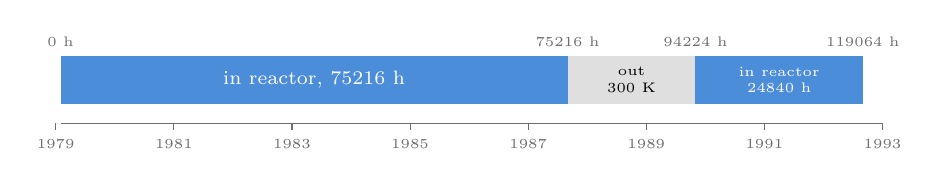
\begin{tikzpicture}[x=0.75cm, y=1cm, >={Stealth[length=2mm]}]
    % years axis 1979-1993 (Feb 1979 = 1979.08 at x = 0)
    \def\xa{1979.083}
    \draw[muted] (0,0) -- (13.9,0);
    \foreach \y in {1979,1981,...,1993} \draw[muted] ({\y-\xa},0) -- ++(0,-0.08) node[below, font=\tiny] {\y};
    % in reactor 1: Feb 1979 - Sep 1987; out: Sep 1987 - Nov 1989; in reactor 2: Nov 1989 - Sep 1992
    \fill[new!70] ({1979.083-\xa},0.25) rectangle ({1987.667-\xa},0.85);
    \fill[gray!25] ({1987.667-\xa},0.25) rectangle ({1989.833-\xa},0.85);
    \fill[new!70] ({1989.833-\xa},0.25) rectangle ({1992.667-\xa},0.85);
    \node[font=\scriptsize, white] at ({(1979.083+1987.667)/2-\xa},0.55) {in reactor, 75216 h};
    \node[font=\tiny, align=center] at ({(1987.667+1989.833)/2-\xa},0.55) {out\\300 K};
    \node[font=\tiny, white, align=center] at ({(1989.833+1992.667)/2-\xa},0.55) {in reactor\\24840 h};
    \foreach \t/\h in {1979.083/0, 1987.667/75216, 1989.833/94224, 1992.667/119064}
      \node[font=\tiny, muted, above] at ({\t-\xa},0.85) {\h\ h};
  \end{tikzpicture}
  \par\medskip
  \begin{columns}[T]
    \begin{column}{0.53\textwidth}
      \scriptsize
      \begin{itemize}
        \item \NEW{continuous operation in the two periods of the paper (p.\,237), 100056 h in reactor; between them $F = 0$, 300 K}
        \item \NEW{constant $F = 5.003\times10^{18}$ fiss/(m$^3$ s) $\Rightarrow$ 62.41 MWd/kgUO$_2$ = 70.8 GWd/tHM at the end:
          70.80 GWd/MTU is the \emph{maximum} burnup of the specimens, so an upper bound}
        \item \NEW{four rings of equal volume, $(r/R)^2$ = 0.125, 0.375, 0.625, 0.875, uniform $F$ (no rim peak)}
        \item \NEW{parabolic profile $T(r) = T_s + (T_c - T_s)[1 - (r/R)^2]$, $T_c = 900\,^\circ$C (below the 1200\,$^\circ$C of p.\,237),
          $T_s = 450\,^\circ$C (rim 400--500\,$^\circ$C, p.\,237), constant in time}
        \item grain radius 15 $\mu$m (grain size 30 $\mu$m), 3.0\% U-235; other settings as the calibration cases
      \end{itemize}
    \end{column}
    \begin{column}{0.44\textwidth}
      \centering\footnotesize
      \renewcommand{\arraystretch}{1.1}
      \begin{tabular}{@{}lccc@{}}
        \toprule
        Case & $r/R$ & $T$ (K) & $T$ ($^\circ$C) \\
        \midrule
        \texttt{Buck2015\_r035} & 0.354 & 1117 & 844 \\
        \texttt{Buck2015\_r061} & 0.612 & 1004 & 731 \\
        \texttt{Buck2015\_r079} & 0.791 & 892 & 619 \\
        \texttt{Buck2015\_r094} & 0.935 & 779 & 506 \\
        \bottomrule
      \end{tabular}\par\medskip
      {\scriptsize cases \texttt{test\_FMP\_UO2\_Buck2015\_*}\\ regression group \texttt{-{}-metallicinclusions}}
    \end{column}
  \end{columns}
\end{frame}

% =====================================================================================================
\begin{frame}{ATM-109: how the model is compared with Fig.\,6}
  \small
  \begin{itemize}
    \item Fig.\,6 (p.\,240): cumulative number fraction vs $\ln V$ ($V$ in nm$^3$) for the two dissolutions; \NEW{digitized}
      (\texttt{data/buck2015/fig6\_*.txt}, binned marker pixels, approximate)
    \item \NEW{log-normal fit of $\ln V$} (\texttt{data/buck2015/summary.txt}); diameter of the equivalent sphere $d = (6V/\pi)^{1/3}$:
      \[\NEW{\ln d \sim \mathcal{N}\!\left(\mu_d, \sigma_d\right),\quad \mu_d = \frac{\mu_{\ln V} + \ln(6/\pi)}{3},\quad \sigma_d = \frac{\sigma_{\ln V}}{3},\quad
      d_{\mathrm{median}} = e^{\mu_d},\quad \bar d = e^{\mu_d + \sigma_d^2/2}}\]
    \item the fits give number-mean diameters of 50 and 62 nm, close to the 43 and 58 nm of the text: \NEW{the reported values look
      like number means}
    \item \NEW{model: pellet-averaged population, the four rings with equal volume, intragranular and grain-boundary particles
      weighted by number ($N_{\mathrm{intra}}$, $N_{\mathrm{GB}}$); one size per ring and population}
  \end{itemize}
  \begin{center}\footnotesize
  \begin{tabular}{@{}lccc@{}}
    \toprule
    & $\mu_{\ln V}$, $\sigma_{\ln V}$ & median $d$ (nm) & number-mean $d$ (nm) \\
    \midrule
    carbonate-peroxide & 7.07, 4.90 & 13 & 50 (reported 43) \\
    nitric acid & 9.30, 3.83 & 28 & 62 (reported 58) \\
    \bottomrule
  \end{tabular}
  \end{center}
\end{frame}

% =====================================================================================================
\begin{frame}{ATM-109: results}
  \centering
  \includegraphics[width=0.86\textwidth]{buck2015_ATM109.png}\par\smallskip
  \begin{columns}[T]
    \begin{column}{0.47\textwidth}
      \scriptsize
      \renewcommand{\arraystretch}{1.0}
      \begin{tabular}{@{}lcccc@{}}
        \toprule
        Ring & $d_{\mathrm{intra}}$ & $d_{\mathrm{GB}}$ & metal & metal in \\
        & (nm) & (nm) & dissolved & GB part. \\
        \midrule
        0.35, 1117 K & 20.3 & 35.5 & 8\% & 2.32\% \\
        0.61, 1004 K & 15.0 & 26.2 & 14\% & 1.90\% \\
        0.79, 892 K & 11.3 & 19.7 & 34\% & 1.39\% \\
        0.94, 779 K & 7.2 & 12.6 & 93\% & 0.16\% \\
        \bottomrule
      \end{tabular}
    \end{column}
    \begin{column}{0.5\textwidth}
      \scriptsize
      \renewcommand{\arraystretch}{1.0}
      \begin{tabular}{@{}lccc@{}}
        \toprule
        & median $d$ & mean $d$ & mean $\ln V$ \\
        & (nm) & (nm) & ($V$ in nm$^3$) \\
        \midrule
        Buck, carbonate-peroxide & 13 & 50 (43) & 7.07 \\
        Buck, nitric acid & 28 & 62 (58) & 9.30 \\
        \MOD{SCIANTIX, two zones} & 11 & 12.5 & 6.78 \\
        SCIANTIX, VB parameters & 19 & 18.5 & 7.95 \\
        \bottomrule
      \end{tabular}
    \end{column}
  \end{columns}
  \par\smallskip
  {\scriptsize Median just below the carbonate-peroxide series; number mean 3.5--5 times too low; distribution much narrower (one size
  per ring and population), the 100--300 nm particles are missing; GB particles (26--36 nm in the inner rings) closer, but 2\% of the particles.}
\end{frame}

% =====================================================================================================
\begin{frame}{Thermochemistry cases: setup and results}
  \small
  \texttt{thermochemistry/test\_FMP\_UO2\_OC\_*}: the calibration cases with \texttt{iThermochimica = 2} (OpenCalphad at every step),
  \texttt{iStoichiometryDeviation = 7} (Kleykamp 1979, same $x$(burnup) at the four positions), Blackburn oxygen potential,
  $p = 10^5$ Pa. Regression group \texttt{-{}-metallicinclusions-oc -{}-oc}.
  \begin{center}\footnotesize
  \renewcommand{\arraystretch}{1.1}
  \begin{tabular}{@{}lcccccc@{}}
    \toprule
    & $\mu_{\mathrm{O_2}}$ & $x$ & Mo & $R_{\mathrm{intra}}$ (nm) & $R_{\mathrm{GB}}$ (nm) & $R_{\mathrm{GB}}$ (nm) \\
    $r/R$ & (kJ/mol) & & oxidised & OC / no OC & OC / no OC & TEM \\
    \midrule
    0.00 & $-375$ & $1.4\times10^{-5}$ & 32\% & 7.1 / 7.6 & 12.4 / 13.2 & 14.3 \\
    0.30 & $-384$ & $6.6\times10^{-6}$ & 33\% & 6.4 / 6.8 & 11.2 / 12.0 & 12.0 \\
    0.56 & $-402$ & $1.0\times10^{-6}$ & 43\% & 4.8 / 5.3 & 8.5 / 9.3 & 5.6 \\
    0.75 & $-265$ & $5.8\times10^{-3}$ & 100\% & 2.7 / 3.6 & 4.8 / 6.2 & 6.7 \\
    \bottomrule
  \end{tabular}
  \end{center}
  \begin{itemize}\footnotesize
    \item \NEW{$r/R$ = 0--0.56: fuel buffered at Mo/MoO$_2$}, $x$ far below Kleykamp ($8.7\times10^{-3}$, $-255$ kJ/mol, all Mo oxidised without the balance)
    \item \NEW{$r/R$ = 0.75: 89\% of the metal dissolved, the particle Mo is not enough, all oxidised; $x$ rises with burnup}
    \item OpenCalphad: MoO$_2$, HCP\_A3 and BCC\_A2 (metal), Mo$_4$O$_{11}$ at some steps; at a few steps no convergence
      (previous $f_{\mathrm{ox}}$ kept); in r000 the convergence of one step can change between runs (final values within $10^{-5}$)
  \end{itemize}
\end{frame}

% =====================================================================================================
\begin{frame}{Thermochemistry cases: evolution}
  \centering
  \includegraphics[width=0.8\textwidth]{fmp_thermochemistry.png}\par
  \small (a, b) oxygen potential and $x$ with the oxygen balance (thick) and Kleykamp only (thin); (c) Mo oxidised; (d) phases at
  the grain boundary; (e) $R_{\mathrm{GB}}$ with and without OpenCalphad vs TEM; (f) share of the excess oxygen in the Mo oxides.
\end{frame}

% =====================================================================================================
\begin{frame}{Verification, 4 November 2026}
  \small
  \begin{itemize}
    \item \textbf{Regression} (\texttt{python3 -m testing.runner -{}-metallicinclusions -{}-metallicinclusions-oc -{}-oc}):
      \textbf{12 passed, 0 failed} --- 4 calibration cases, 4 ATM-109 rings, 4 thermochemistry cases; build up to date with the sources
    \item \textbf{Calibration still valid}: model of the calibration copy = current code (only the 4 parameter lines differ);
      $J_4$ = 0.5541 recomputed with the parameters in the code; $\pm5\%$ on each parameter increases $J_4$ (local minimum)
    \item \textbf{Mass conservation}: $C_{m1} + C_{m2} + C^{\mathrm{intra}} + C^{\mathrm{GB}} = \sum_X C_X^{\mathrm{prod}}$ within
      $4\times10^{-7}$ (output precision) in r000, r075, ATM-109 r035
    \item \textbf{Exchange}: $k_{\mathrm{GB}}^2$ analytical vs finite volumes within $6\times10^{-8}$ (\texttt{check\_exchange.py})
    \item all the changes tagged \texttt{EC November 2026} in the code; documentation in \texttt{validation/metallicinclusions/README.md}
  \end{itemize}
\end{frame}

% =====================================================================================================
\begin{frame}{Known limits and open points}
  \small
  \begin{itemize}
    \item $f_{A,\mathrm{intra}}$ 4--10 times TEM at $r/R$ = 0--0.30, 2 times too low at 0.75: the intragranular number density is the
      main remaining discrepancy
    \item $R_{\mathrm{GB}}$ too large at $r/R$ = 0.56 (9.3 vs 5.6 nm)
    \item at low temperature most of the metal stays dissolved (89\% at $r/R$ = 0.75, 93\% in the outer ATM-109 ring)
    \item one mean size per population: no size distribution; ATM-109 mean size underestimated (12.5 vs 43--58 nm)
    \item \NEW{$K_{\mathrm{ex}}$ [TBC]: zone 2 as a well-mixed layer, $D_{\mathrm{intra}}$ also in zone 2}
    \item \textbf{inputs inherited from V.\,Bellani}: grain radius 12.3 $\mu$m and 4.0\% U-235, while thesis Tab.\,5.1 reports a mean grain
      size of 8.8 $\mu$m and 4.48\% U-235 ($a$ enters $\phi_2$, $N_{\mathrm{site,GB}}$, $K_{\mathrm{ex}}$: a change needs a new calibration)
    \item calibration without OpenCalphad (the Mo oxidation reduces the radii by 5--25\%)
    \item oxygen balance: only the particle Mo takes oxygen, excess oxygen from Kleykamp, no radial O/M
    \item lumped species: particle composition = production composition (measured particles poorer in Mo, richer in Ru)
    \item MOX systems keep fast-reactor yields: validated only for UO$_2$ in LWR conditions
  \end{itemize}
\end{frame}

% =====================================================================================================
\begin{frame}{References}
  \scriptsize
  \begin{itemize}
    \item[{[VB]}] V.\,Bellani, \emph{Modelling of nucleation and growth of metallic fission product inclusions in irradiated UO$_2$ fuel with
      neutronics-based source terms for SCIANTIX implementation}, MSc thesis, Politecnico di Milano, 2025--2026.
    \item E.C.\,Buck, E.J.\,Mausolf, B.K.\,McNamara, C.Z.\,Soderquist, J.M.\,Schwantes, \emph{Nanostructure of metallic particles in light water
      reactor used nuclear fuel}, J.\,Nucl.\,Mater.\ 461 (2015) 236--243.
    \item S.F.\,Wolf, D.L.\,Bowers, J.C.\,Cunnane, J.\,Radioanal.\,Nucl.\,Chem.\ 263 (2005) 581--586 (ATM-109, ref.\ [21] of Buck et al.).
    \item M.\,Angleraud, PhD thesis, Université de Toulouse, 2024 (TEM data of the calibration, ref.\ [13] of [VB]).
    \item A.D.\,Brailsford, R.\,Bullough, \emph{The theory of sink strengths}, Phil.\,Trans.\,R.\,Soc.\,Lond.\ A 302 (1981) 87--137,
      doi:10.1098/rsta.1981.0158.
    \item A.D.\,Brailsford, R.\,Bullough, M.R.\,Hayns, J.\,Nucl.\,Mater.\ 60 (1976) 246--256; F.S.\,Ham, J.\,Phys.\,Chem.\,Solids 6 (1958) 335--351.
    \item A.H.\,Booth, AECL-496 (CRDC-721), Atomic Energy of Canada Limited, 1957.
    \item H.\,Kleykamp, J.\,Nucl.\,Mater.\ 131 (1985) 221--246 (solubility); H.\,Kleykamp, \emph{The chemical state of LWR high-power rods under
      irradiation}, J.\,Nucl.\,Mater.\ (1979) (stoichiometry, \texttt{iStoichiometryDeviation = 7}).
    \item P.E.\,Blackburn, J.\,Nucl.\,Mater.\ 46 (1973) 244--252.
    \item G.\,Brillant, F.\,Gupta, A.\,Pasturel, J.\,Phys.: Condens.\ Matter 21 (2009) 285602.
    \item M.S.\,Veshchunov, V.E.\,Shestak, J.\,Nucl.\,Mater.\ 384 (2009) 12--18.
    \item S.\,Sakib et al., J.\,Nucl.\,Mater.\ 614 (2025) 155859.
    \item D.\,Kashchiev, \emph{Nucleation: Basic Theory with Applications}, Butterworth-Heinemann, 2000.
  \end{itemize}
\end{frame}

\end{document}
